\documentclass[12pt,a4paper]{article}

\usepackage[utf8]{inputenc}
\usepackage[T2A]{fontenc}
\usepackage[ukrainian]{babel}
\usepackage{geometry}
\usepackage{amsmath}
\usepackage{array}
\usepackage{multirow}
\usepackage[table]{xcolor}
\usepackage{makecell}
\usepackage{graphicx}
\usepackage{fancyvrb}
\usepackage{hyperref}

\geometry{
    left=2cm,
    right=2cm,
    top=2cm,
    bottom=2cm
}

\setlength{\parindent}{1.25cm}
\setlength{\parskip}{0.2em}
\setlength{\extrarowheight}{2pt}

\newcolumntype{C}[1]{>{\centering\arraybackslash}p{#1}}
\newcommand{\sectiontitle}[1]{\begin{center} \textbf{\large #1} \end{center}}
\fvset{frame=single, framesep=2mm, fontsize=\small}

\hypersetup{
    unicode=true,
    pdftitle={ІО-41, Давидчук А.М., АК. Частина 1, Лабораторна робота №4},
    pdfauthor={Давидчук Артем},
    pdfsubject={Архітектура Комп'ютерів. Частина 1}
}

\begin{document}

\hypersetup{pageanchor=false}
\begin{titlepage}

        \begin{center}
\includegraphics[width=0.7\textwidth]{../../../TITLES/letterhead.png}\end{center}

        \begin{center}
            \large Національний технічний університет України\\
            «Київський політехнічний інститут імені Ігоря Сікорського»\\[1em]
            Факультет інформатики та обчислювальної техніки\\
            Кафедра обчислювальної техніки
        \end{center}

        \vfill

        \begin{center}
            \textbf{\LARGE Архітектура Комп'ютерів. Частина 1}\\[2em]
            \textbf{\Large Лабораторна робота №4}\\[0.5em]
            «Обробка інформації в ЕОМ на програмному і мікропрограмному рівнях»
        \end{center}

        \vfill

        \begin{flushright}
            Виконав: студент 2 курсу ФІОТ, гр. ІО-41\\
            \textit{Давидчук А. М.}\\
            Залікова книжка № 4106\\[1em]
            Перевірив: \textit{Верба О.\,А.}
        \end{flushright}

        \vfill

        \begin{center}Київ --- 2026\end{center}

    \end{titlepage}
\hypersetup{pageanchor=true}

    \noindent
    \textbf{\underline{Тема:}} «Обробка інформації в ЕОМ на програмному і мікропрограмному рівнях».

    \vspace{1em}


\noindent
\textbf{\underline{Мета:}} вивчити етапи формування системи команд процесорів, різновиди
форматів команд та способів адресації операндів. Навчитися розробляти
мікроалгоритми і мікропрограми виконання етапів команд з використанням
мнемонічного мікроасемблера.

\begin{center} \textbf{\large Хід роботи} \end{center}

\sectiontitle{Підготовка до роботи}

Номер варіанту -- $4106_{10} = 0001\ 0000\ 0000\ 1010_2$.

\[
a_7 = 0,\quad a_6 = 0,\quad a_5 = 0,\quad a_4 = 1,\quad
a_3 = 0,\quad a_2 = 1,\quad a_1 = 0.
\]

\begin{center}
\small
\begin{minipage}[t]{0.47\textwidth}
\centering
\resizebox{\linewidth}{!}{
\begin{tabular}{|C{1.1cm}|C{1.1cm}|C{1.1cm}|C{3.8cm}|}
    \hline
    $a_3$ & $a_2$ & $a_1$ & Операція \\
    \hline
    0 & 0 & 0 & $X + Y$ \\
    \hline
    0 & 0 & 1 & $X - Y$ \\
    \hline
    \rowcolor{yellow!25}
    0 & 1 & 0 & $X \& Y$ \\
    \hline
    0 & 1 & 1 & $X \vee Y$ \\
    \hline
\end{tabular}
}
\end{minipage}
\hfill
\begin{minipage}[t]{0.47\textwidth}
\centering
\resizebox{\linewidth}{!}{
\begin{tabular}{|C{1.1cm}|C{1.1cm}|C{1.1cm}|C{1.5cm}|C{1.5cm}|}
    \hline
    $a_7$ & $a_6$ & $a_5$ & РС & РД \\
    \hline
    \rowcolor{yellow!25}
    0 & 0 & 0 & 02H & 04H \\
    \hline
    0 & 0 & 1 & 12H & 14H \\
    \hline
    0 & 1 & 0 & 22H & 24H \\
    \hline
    0 & 1 & 1 & 32H & 34H \\
    \hline
\end{tabular}
}
\end{minipage}

\vspace{1.2em}

\begin{minipage}[t]{0.47\textwidth}
\centering
\resizebox{\linewidth}{!}{
\begin{tabular}{|C{1.6cm}|C{5.5cm}|}
    \hline
    $a_4$ & Тип адресації \\
    \hline
    0 & Пряма \\
    \hline
    \rowcolor{yellow!25}
    1 & Пряма регістрова \\
    \hline
\end{tabular}
}
\end{minipage}
\hfill
\begin{minipage}[t]{0.47\textwidth}
\centering
\resizebox{\linewidth}{!}{
\begin{tabular}{|C{1.4cm}|C{1.4cm}|C{4.9cm}|}
    \hline
    $a_2$ & $a_1$ & Спосіб множення \\
    \hline
    0 & 0 & 1-й \\
    \hline
    0 & 1 & 2-й \\
    \hline
    \rowcolor{yellow!25}
    1 & 0 & 3-й \\
    \hline
    1 & 1 & 4-й \\
    \hline
\end{tabular}
}
\end{minipage}
\end{center}
\normalsize

Для обрахунків оберемо такі значення:
\[
X = 14,\qquad Y = 11,\qquad Z = 5.
\]

\newpage

\sectiontitle{Структура ЕОМ}

\begin{center}
    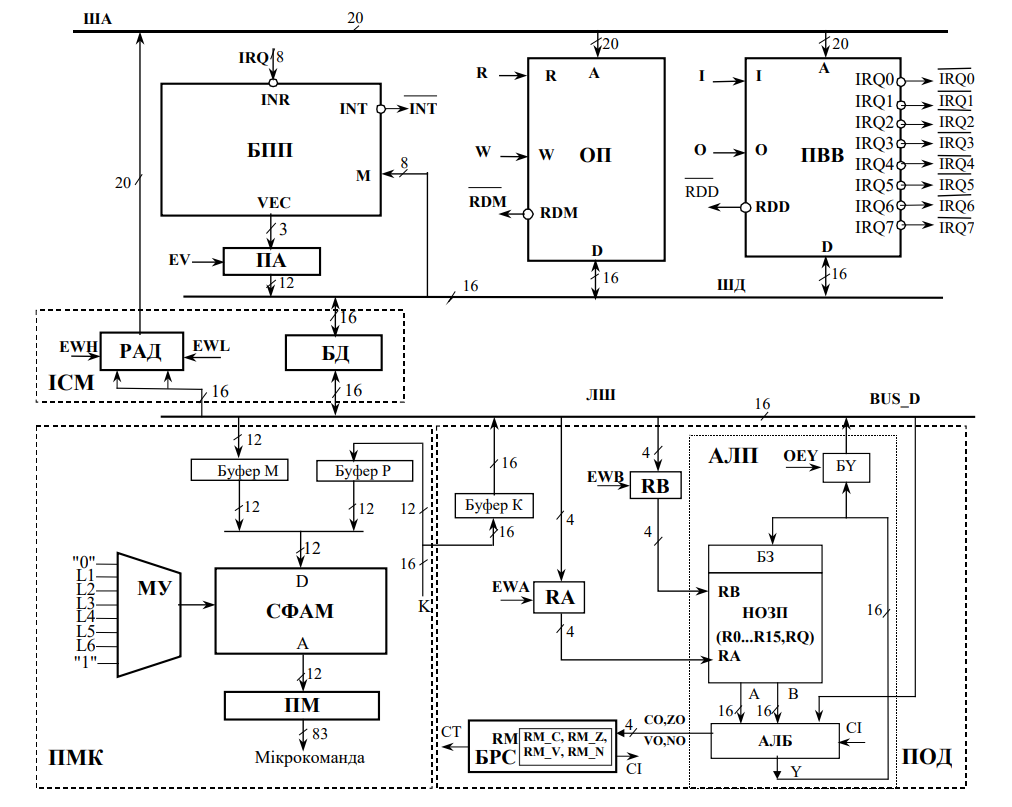
\includegraphics[width=0.82\textwidth]{../lab3/media/eom.png}
\end{center}

\sectiontitle{Формат одноадресних команд та формат регістрів стану і даних}

\begin{center}
\small
\begin{tabular}{|C{2.2cm}|C{2.5cm}|C{2cm}|C{7cm}|}
    \hline
    \textbf{Поле} & \textbf{Біти} & \textbf{Довжина} & \textbf{Призначення} \\
    \hline
    $F$ & 15 & 1 & формат команди \\
    \hline
    $OP$ & 14--11 & 4 & код операції \\
    \hline
    $TA$ & 10 & 1 & тип адресації: 0 -- пряма, 1 -- пряма регістрова \\
    \hline
    $A$ & 9--0 & 10 & адреса ОП або номер регістра/порту \\
    \hline
\end{tabular}
\end{center}

\begin{center}
\small
\begin{tabular}{|C{1.6cm}|C{10cm}|}
    \hline
    \textbf{Регістр} & \textbf{Призначення} \\
    \hline
    РС & 7-й біт містить ознаку готовності пристрою до обміну даними \\
    \hline
    РД & містить дані, що зчитуються із зовнішнього пристрою \\
    \hline
\end{tabular}
\end{center}
\normalsize

\newpage

\sectiontitle{Архітектура системи}

\begin{center}
\begin{minipage}[t]{0.47\textwidth}
\centering
\textbf{Структура НОЗП}

\vspace{0.4em}
\small
\begin{tabular}{|C{1.8cm}|p{4.5cm}|}
    \hline
    \textbf{Регістр} & \textbf{Призначення} \\
    \hline
    R1 & стан порту \\
    \hline
    R2 & операнд $X$ \\
    \hline
    R3 & лічильник команд \\
    \hline
    R4 & поточна команда \\
    \hline
    R5 & операнд $Y$ \\
    \hline
    R6 & операнд $Z$ \\
    \hline
    R7 & результат $X \& Y$ \\
    \hline
    R8 & множене \\
    \hline
    R9 & старші біти результату \\
    \hline
    R10 & молодші біти результату \\
    \hline
    R11 & лічильник циклів \\
    \hline
\end{tabular}
\end{minipage}
\hfill
\begin{minipage}[t]{0.47\textwidth}
\centering
\textbf{Структура ПМК}

\vspace{0.4em}
\small
\begin{tabular}{|C{1.5cm}|p{4.7cm}|}
    \hline
    \textbf{Адреса} & \textbf{Мікропрограма} \\
    \hline
    0h & старт \\
    \hline
    1h & test \\
    \hline
    2h & ready\_test \\
    \hline
    3h & input \\
    \hline
    4h & load\_y \\
    \hline
    5h & load\_z \\
    \hline
    6h & op\_xy \\
    \hline
    7h & multiply \\
    \hline
    8h & write \\
    \hline
    9h & end \\
    \hline
\end{tabular}
\end{minipage}
\end{center}

\vspace{1em}

\begin{center}
\begin{minipage}[t]{0.47\textwidth}
\centering
\textbf{Структура ОП}

\vspace{0.4em}
\small
\begin{tabular}{|C{1.5cm}|p{4.8cm}|}
    \hline
    \textbf{Адреса} & \textbf{Вміст} \\
    \hline
    1h & значення $Y$ \\
    \hline
    2h & значення $Z$ \\
    \hline
    3h & старше слово результату \\
    \hline
    4h & молодше слово результату \\
    \hline
    20h--28h & програма \\
    \hline
\end{tabular}
\end{minipage}
\hfill
\begin{minipage}[t]{0.47\textwidth}
\centering
\textbf{Структура ЗП}

\vspace{0.4em}
\small
\begin{tabular}{|C{1.5cm}|p{4.8cm}|}
    \hline
    \textbf{Адреса} & \textbf{Вміст} \\
    \hline
    02h & РС \\
    \hline
    04h & РД \\
    \hline
\end{tabular}
\end{minipage}
\end{center}

\newpage

\sectiontitle{Змістовний мікроалгоритм}

\begin{center}

\includegraphics[width=0.42\textwidth]{media/alg.png}
\end{center}

\sectiontitle{Система команд}

\begin{center}
\small
\begin{tabular}{|C{2.5cm}|C{2cm}|p{8cm}|}
    \hline
    \textbf{Команда} & \textbf{Код програми} & \textbf{Операція} \\
    \hline
    \texttt{test} & 1h & тестування готовності порту \\
    \hline
    \texttt{ready\_test} & 2h & перевірка біта готовності пристрою \\
    \hline
    \texttt{input} & 3h & введення значення $X$ з РД \\
    \hline
    \texttt{load\_y} & 4h & зчитування операнда $Y$ з ОП \\
    \hline
    \texttt{load\_z} & 5h & зчитування операнда $Z$ з ОП \\
    \hline
    \texttt{op\_xy} & 6h & виконання операції $X \& Y$ \\
    \hline
    \texttt{multiply} & 7h & множення результату $X \& Y$ на $Z$ \\
    \hline
    \texttt{write} & 8h & запис результату множення в ОП \\
    \hline
    \texttt{end} & 9h & завершення мікропрограми \\
    \hline
\end{tabular}
\end{center}

\sectiontitle{Обрахунки}
\[
X = 14_{10} = 00.00\ 0000\ 0000\ 1110_2 = 000E_{16},
\]
\[
Y = 11_{10} = 00.00\ 0000\ 0000\ 1011_2 = 000B_{16},
\]
\[
Z = 5_{10} = 00.00\ 0000\ 0000\ 0101_2 = 0005_{16},
\]
\[
X \& Y = 14_{10} \& 11_{10} = 10_{10} = 000A_{16},
\]
\[
F = (X \& Y) \times Z = 10_{10} \times 5_{10} = 50_{10} = 0032_{16}.
\]

\sectiontitle{Мікропрограма}

\VerbatimInput{project/LAB4.ASM}

\sectiontitle{Результат виконання}
\[
F = (X \& Y) \times Z = 50_{10} =
00.00\ 0000\ 0000\ 0000\ 0000\ 0000\ 0011\ 0010_2 = 0000\ 0032_{16}
\]

\noindent
Після виконання мікропрограми в оперативній пам'яті мають бути записані:

\begin{center}
\begin{tabular}{|C{3cm}|C{4cm}|}
    \hline
    \textbf{Адреса} & \textbf{Значення} \\
    \hline
    \texttt{M[3h]} & \texttt{0000h} \\
    \hline
    \texttt{M[4h]} & \texttt{0032h} \\
    \hline
\end{tabular}
\end{center}

\noindent
І так, запустимо DosBox:

\begin{center}
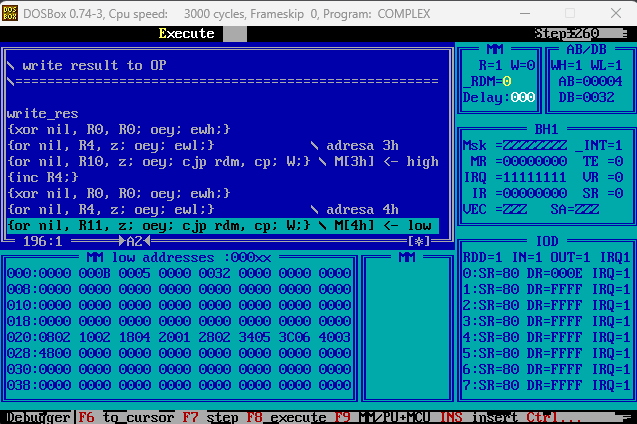
\includegraphics[width=0.8\textwidth]{media/program.png}
\end{center}

\noindent
Як бачимо, значення співпали.

\sectiontitle{Висновок}

У результаті виконання лабораторної роботи було сформовано
структуру системи, визначено варіант завдання та побудовано змістовний
мікроалгоритм обробки даних. Для мого варіанта реалізовано операцію
$F = (X \& Y) \times Z$, де операнд $X$ надходить із зовнішнього пристрою,
операнди $Y$ і $Z$ зчитуються з оперативної пам'яті, а результат записується назад в
ОП. Було складено систему команд, виконано ручні обрахунки та підготовлено
мікропрограму, яка відображає етапи тестування пристрою, вводу даних,
обчислення логічної операції, множення та запису результату.

\newpage

\sectiontitle{Відповіді на контрольні питання}

\begin{enumerate}
    \item \textbf{Охарактеризуйте етапи виконання команд основної групи, передачі
    керування, введення-виведення, системних.}

    Команди основної групи виконуються через вибірку команди, дешифрування,
    вибірку операндів, виконання операції та запис результату. Для команд передачі
    керування додатково аналізується умова переходу та змінюється лічильник команд.
    Для команд введення-виведення виконується обмін із портами пристроїв та
    перевірка сигналів готовності. Системні команди змінюють режими роботи
    процесора, стан переривань або службові параметри системи.

    \item \textbf{Охарактеризуйте основні способи адресації операндів з використанням і без використання РЗП.}

    Без використання РЗП застосовують пряму, непряму та безпосередню адресації.
    Пряма адресація задає точну адресу операнда, непряма використовує адресу
    вказівника, а безпосередня містить сам операнд у полі команди. З використанням
    РЗП реалізують пряму регістрову, базову та індексну адресації, де виконавча
    адреса або сам операнд визначаються через регістри загального призначення.

    \item \textbf{Як забезпечити правильне зчитування і запис даних у пам'ять з урахуванням швидкодії пам'яті?}

    Для цього використовують сигнали готовності пам'яті та цикли очікування.
    Після подачі сигналу читання або запису процесор повинен дочекатися сигналу
    \texttt{RDM}. Якщо доступ повільний, у мікропрограмі вводяться додаткові такти
    очікування, які узгоджують роботу пам'яті та процесора.

    \item \textbf{Яким чином можна керувати записом інформації в RA і RB, навіщо використовуються зазначені регістри?}

    Запис у RA і RB виконується спеціальними керуючими сигналами, які подаються
    з ПМК. Ці регістри використовуються для вибору операндів у НОЗП та організації
    доступу до двох джерел даних одночасно. Через них задаються адреси регістрів,
    які підключаються до входів арифметико-логічного блока.

    \item \textbf{Поясніть призначення директив мікроасемблера, які визначають роботу з пам'яттю.}

    Директива \texttt{ORG} задає адресу розміщення мікрокоманд, \texttt{DW}
    використовується для ініціалізації комірок пам'яті, \texttt{ACCEPT} задає
    початковий стан регістрів, пам'яті та зовнішніх пристроїв, а \texttt{LINK}
    визначає конфігурацію зв'язків між шинами, регістрами та входами ПМК.

    \item \textbf{Як забезпечити обмін даними між процесором і ЗП в програмному режимі?}

    У програмному режимі процесор звертається до регістрів стану і даних зовнішнього
    пристрою через відповідні адреси портів. Спочатку перевіряється біт готовності в
    РС, після чого виконується читання або запис через РД. Такий підхід дозволяє
    уникнути конфлікту між швидкодією процесора і зовнішнього пристрою.
\end{enumerate}

\end{document}
